\subsection{Quest\~{a}o de Pesquisa 1}
\emph{Quais as áreas de SOC são mais frequentemente pesquisadas no contexto de qualidade de serviços?}

%A QP2 tem como objetivo trazer uma perspectiva do cen\'{a}rio das pesquisas em Computa\c{c}\~{a}o Orientada a Servi\c{c}o com foco em QoS atualmente. Para responder a essa pergunta, precisamos primeiramente definir quais s\~{a}o as \'{a}reas que melhor caracterizam as diversas contribui\c{c}\~{o}es de pesquisa em SOC. Da\'{i} ent\~{a}o realizamos a classifica\c{c}\~{a}o.

Para responder a essa pergunta primeiramente identificamos as principais caracter\'{i}sticas de SOC. Encontramos no projeto europeu S-Cube a fundamenta\c{c}\~{a}o mais clara para definir tais caracter\'{i}sticas~\cite{SCube-FINALREPORT} e, portanto, o adotamos como refer\^{e}ncia para definição da faceta da contribui\c{c}\~{a}o. Visando atender ao foco desse estudo, no entanto, adaptamos a estrutura definida no projeto S-Cube, uma vez definido que o presente MS não irá abranger estudos que tratem, em específico, da infraestrutura de soluções baseadas e serviços.

%e obtivemos as seguintes caracter\'{i}sticas: Ciclo de Vida, Composi\c{c}\~{a}o, Coordena\c{c}\~{a}o \& Comunica\c{c}\~{a}o, Descoberta \& Sele\c{c}\~{a}o, Modelos de QoS, Monitoramento \& Adapta\c{c}\~{a}o. 

A Figura~\ref{fig:bubbleplot-QoSSOC} apresenta o diagrama ilustrando a distribui\c{c}\~{a}o dos artigos no eixo horizontal de SOC, a faceta da contribui\c{c}\~{a}o. Assim como os resultados observados nas outras facetas, vale ressaltar que os atributos mapeados não são mutualmente excludentes, visto que representam partes de SOC. Por exemplo, o artigo~\cite{DBLP:conf/dsn/ZhengL09} lida com composi\c{c}\~{a}o, modelos de QoS \& linguagens, além de monitoramento \& adapta\c{c}\~{a}o. Existe dentre eles alguma sobreposição, notavelmente entre composição \& coordenação. No entanto, notou-se que o termo coordenação também envolve aspectos da comunicação entre provedores e consumidores de serviços em geral, independente de composição de serviços. 

\begin{figure}[htb]
\centering
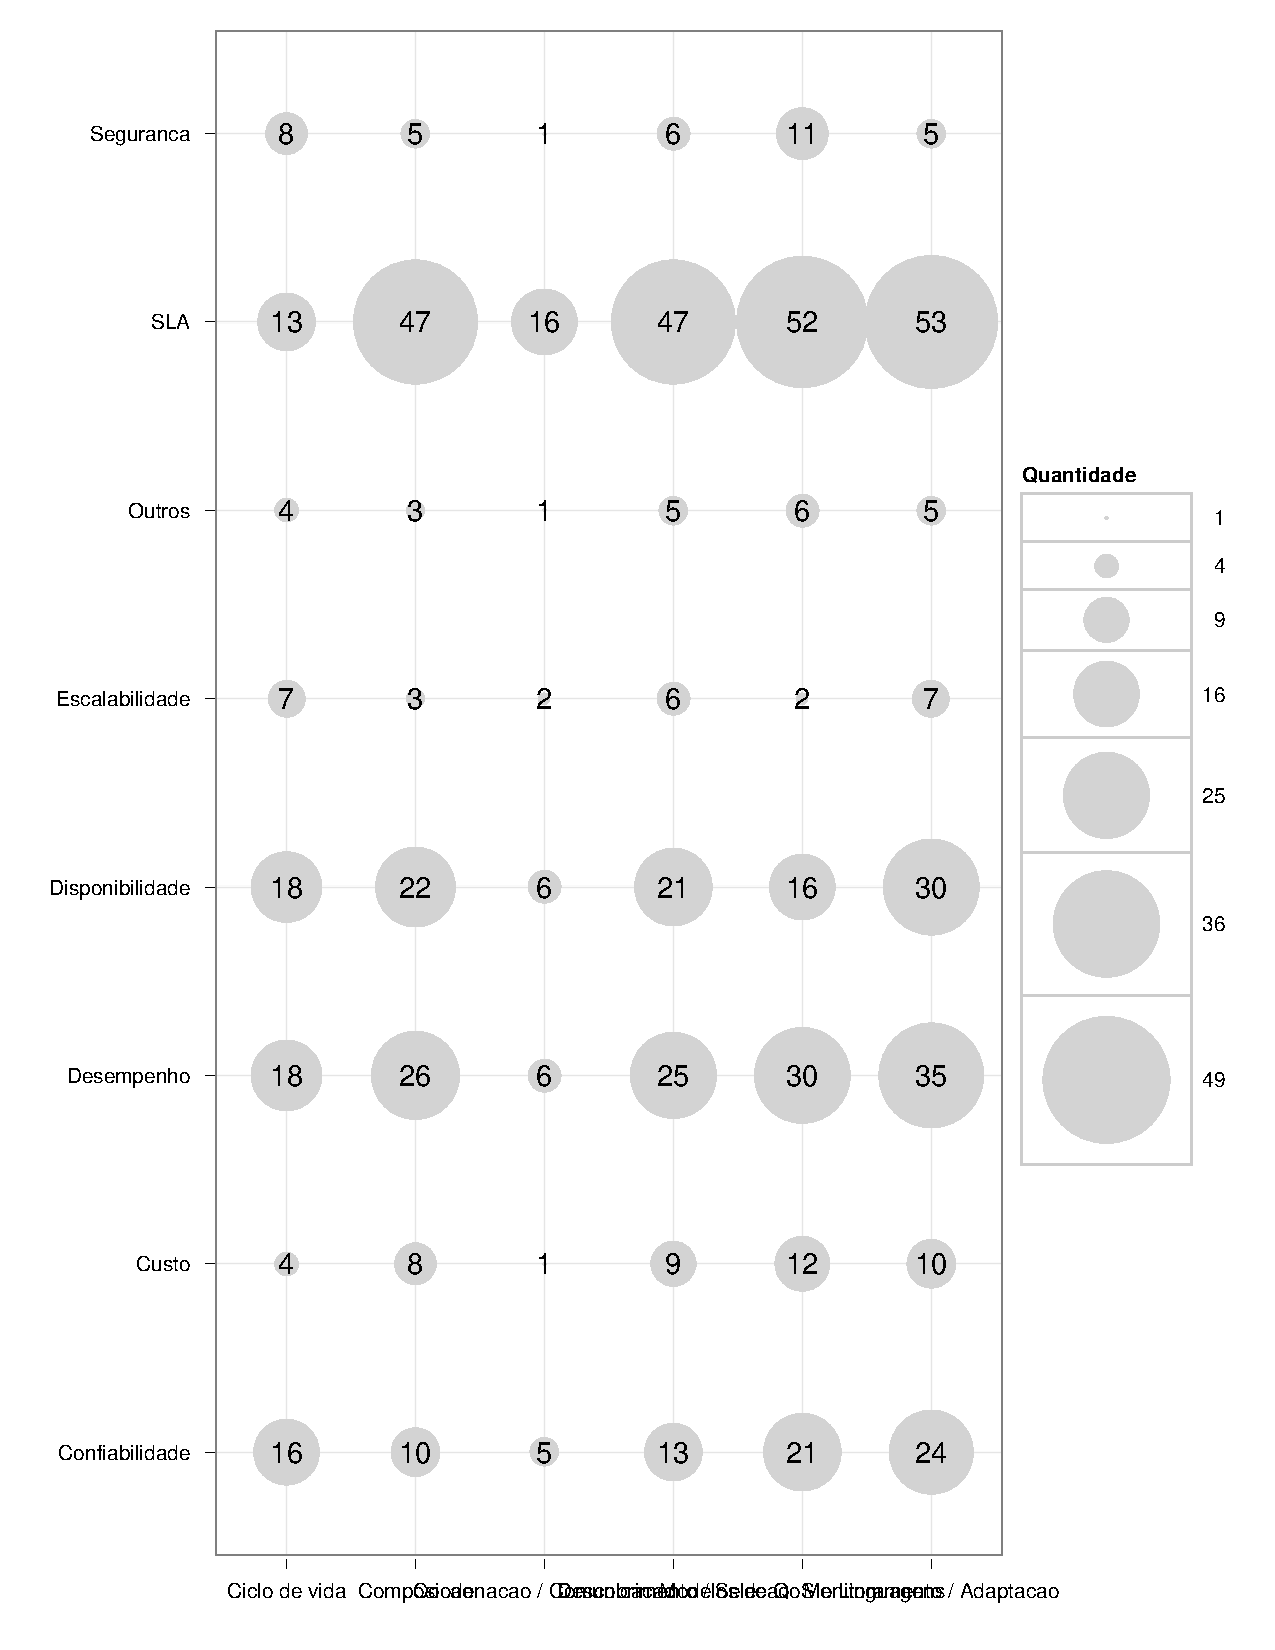
\includegraphics[scale=0.4]{imagens/contribuicaoContexto.pdf}
\caption{\emph{Bubble plot} com a distribui\c{c}\~{a}o ap\'{o}s a realiza\c{c}\~{a}o do primeiro  estudo}
\label{fig:bubbleplot-QoSSOC}
\end{figure}

O resultado desse mapeamento mostra que a maior parte dos trabalhos publicados lida com monitoramento e adapta\c{c}\~{a}o (\MonitoramentoAdaptacao), seguida de modelos de QoS \& linguagens (\ModelosdeQoSeLinguagens), descoberta \& sele\c{c}\~{a}o (\DescobrimentoSelecao),  composi\c{c}\~{a}o (\Composicao), ciclo de vida (\Ciclodevida) e finalmente coordenação & comunicação com \CoodenacaoComunicacao.

Esses resultados indicam o foco dado a aspectos não funcionais, dinâmicos e que podem sofrer variações devido a concorrência e poss\'{i}veis falhas dos servi\c{c}os em tempo de execu\c{c}\~{a}o. Uma preocupa\c{c}\~{a}o que pode refletir problemas no modelo de terceirização de serviços. Uma outra observa\c{c}\~{a}o: dado que o ambiente SOC possui características próprias e diferenciadas, é natural que novas métricas de QoS tenham sido definidas ou que métricas já utilizadas tenham ganhado novos significados, assim como linguagens e especificações que admitam o tratamento e negociação dos requisitos de qualidade. O resultado obtido nesse estudo para o atributo de modelos de QoS e linguagens atesta essa constatação. Nota-se também que a descoberta e seleção de serviços foi bem endereçada nas pesquisas, assim como a composição. No primeiro grupo, é considerado o descobrimento e escolha entre serviços de mesma funcionalidade, porém com diferentes níveis de QoS. O segundo abrange não somente a composição, mas também a escolha da melhor configuração de modo a atender aos níveis globais desejáveis ou necessários de QoS para um conjunto de serviços. Por fim, notou-se um número reduzido de trabalhos que abordam ciclo de vida e menos expressivo ainda com rela\c{c}\~{a}o a coordenação \& comunicação. 